% !TEX root = ../document.tex
% !TeX spellcheck = pt_BR

\section{Proposta de trabalho}
\label{sec:section5}
Até aqui tratamos da implementação das etapas iniciais dos algoritmos -- preprocessamento, extração de características, preparação dos dados --, mas não entramos em questões de classificação. Este será o próximo passo no desenvolvimento do trabalho. Abaixo é apresentada uma proposta de implementação, seguida de um roteiro para validação dos resultados e, por último, um cronograma preliminar de atividades.

\subsection{Implementação}
No caso do método de Rocha et al., a classificação se dará através de duas redes neurais: uma para lidar com a elevação do segmento ST e a outra, com a depressão do segmento ST. A saída será 0 para o caso negativo e 1 para o caso positivo (batida isquêmica). Para obter o resultado final, aplica-se o operador lógico OU à saída das duas redes. Os autores verificaram também que o desempenho de um único sistema de classificação não atinge bons resultados, devido à grande variabilidade morfológica entre ECGs de diferentes derivações\footnote{uma derivação de ECG é um dos possíveis modos de aquisição de atividade elétrica do coração}. Dessa forma, eles propuseram a implementação de um classificador específico para cada derivação.

Ainda no método de Rocha et al. há um último procedimento a ser implementado, que é a detecção de episódios isquêmicos. Nesta etapa, uma janela deslizante é aplicada à lista de batidas do ECG e, se mais de 50\% das batidas nesta janela  forem classificadas como isquêmicas, um novo episódio é detectado. Numa segunda passagem, a detecção é revisada com o objetivo de unir episódios com separação menor que 40 batidas. A figura \ref{fig:rocha_03} ilustra a etapa de classificação.

\begin{figure}[ht]
    \centering
    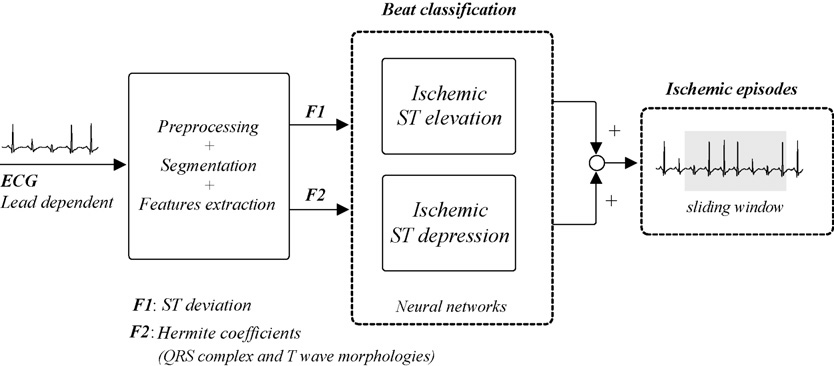
\includegraphics[width=0.8\textwidth]{figures/rocha_03.png}
    \caption{Diagrama de blocos do classificador utilizado no método de Rocha et al. Extraído de \cite{Rocha10}}
    \label{fig:rocha_03}
\end{figure}

No caso do método de Mohebbi e Moghadam \ldots

No caso do método de Gopalakrishnan et al. \ldots

\subsection{Testes e Validação}
Para avaliar a confiabilidade dos algoritmos, lançaremos mão de métricas definidas em termos no número de verdadeiros positivos (VP), verdadeiros negativos (VN), falsos positivos (FP) e falsos negativos (FN) obtidos no teste. Estes conceitos são melhor visualizados numa matriz de confusão, conforme ilustra a tabela \ref{tab:confusion_matrix}.

\begin{table}[ht] 
    \caption{Matriz de confusão}
    \centering
    \begin{tabular}{ccc}
        \toprule
        \multirow{2}{2cm}{Resultado do teste} &
        \multicolumn{2}{c}{Condição real} \\
        \cmidrule{2-3}
        & Presente & Ausente \\ 
        \midrule
        Positivo & VP & FP \\
        \midrule
        Negativo & FN & VN \\
        \bottomrule
    \end{tabular} 
    \label{tab:confusion_matrix}
\end{table} 

Em especial, estamos interessados na sensibilidade ($S_e$) e na preditividade positiva ($P_p$). A sensibilidade diz respeito à probabilidade do teste detectar batidas isquêmicas, enquanto a preditividade positiva pode ser entendida como a probabilidade de um resultado positivo do teste refletir efetivamente a condição testada. Seus valores podem ser obtidos pelas expressões abaixo:
\begin{equation} \label{equ:metrics}
    S_e = \frac{VP}{VP+FN}
    \quad\quad
    P_p = \frac{VP}{FP+VP}
\end{equation}

De modo geral, os conceitos apresentados medem o desempenho de um teste diagnóstico frente a um método de referência. Este método alternativo deve ser confiável e, preferencialmente, realizado por especialistas. Em nosso caso, teremos o diagnóstico dado por cardiologistas que, de maneira unânime, classificaram todas as batidas de todos os registros de ECG num determinado banco de dados. Os bancos utilizados são o European ST-T e o Long-Term ST. Ambos os bancos possuem, independentemente do formato de dados, um campo que indica o diagnóstico das batidas. Neste campo, a letra 'T' indica inversão da onda T, enquanto a letra 's' indica elevação/depressão do segmento ST.

Ao final dos testes, obteremos as medidas necessárias e as compararemos com o resultado publicado nos artigos originais de cada método. Mais importante ainda, compararemos os métodos entre si, e tomaremos uma decisão quanto ao melhor método para ser devidamente implementado e implantado num sistema móvel de monitoramento cardíaco.

Num segundo plano, tentaremos avaliar a eficiência dos algoritmos em termos do tempo de execução. Para tanto, será necessário simular uma configuração de tempo-real, em que as amostras do sinal de ECG são repassadas à entrada do algoritmo uma a uma. Os algoritmos deverão então ser adaptados para armazenar amostras recentes do sinal e descartar a mais antiga quando uma nova é recebida. Dessa forma, trabalhar-se-á com uma janela temporal do sinal de entrada, e uma nova iteração do algoritmo se realizará a cada nova amostra. Entretanto, deve-se salientar que esta não é uma métrica precisa, na medida em que o método escolhido deverá atuar num dispositivo móvel de uso geral. Isto significa que, dependendo  do hardware do dispositivo, um método poderia executar mais rapidamente do que outro, mesmo que a simulação forneça resultado contraditório.


\subsection{Cronograma}
Texto\ldots
